
\chapter{Error Channel}

\lecture{19}{2025-04-29}{Error Correction}{ Petit test pour voir ce que cela écrit}
\begin{parag}{Point to point communication system}
    Now we have compressed the source coding, we encrypted it. What we want now is to actually transfer the message to the receiver side. However we have to protect ourself from the mean world. For example with the communication over the internet it is our application which does the compression and encryption.
\end{parag}


\begin{parag}{Motivation Channel Model}
    The question is how the bad thing happens:
    \begin{itemize}
        \item The internet often drops packets due to congestion
        \item Not all the bits on a storage device can be retrieved
        \item \important{Wireless signals are very noisy}
    \end{itemize}
    We consider two types of channel models:
    \begin{center}
        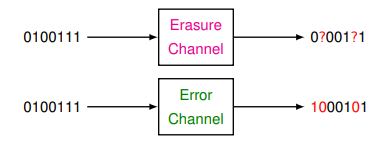
\includegraphics[scale=1]{12025-04-29.png}
    \end{center}
    If we model the world has being a \important{Erasure} channel mode, then the following happens:\\
    So your model replace some of your bit with question mark. (those bit are no longer readable). So for example you store your holiday picture into your hdd but some water fell on it, then there will be some error and those error is the question mark.\\
    The model can \important{only} replace the bit by a question mark.\\
The question is ``how we decide which bit has to be replace with a question mark?'' For example like this:\\
    So for the first $0$ let us say we throw a dice, if the outcome is $6$, we will replace the outcome by a question mark or we won't. Therefore, here we can say that the erosion probability is $\frac{1}{6}$.\\
    However maybe the eraser is not random, maybe someone who know what we're gonna do (the algorithm to find the erasure) will find the one that will be a question mark.\\
Here the channel input alphabet is not necessarily binary.\\
We can take for the alphabet $\mathcal{A} = \{0, 1, 2, 3, 4\}$ and works with this.\\
For the second model (Error Channel), The channel can completely change entire symbol. The output is in the same alphabet as the input (which make the thing ``easier''). What we can do is the substitute (0 to 1, 1 to 0 and then 0 to 0).\\
This makes the channel way harder to know which of these bits have been flipped.
\begin{framedremark}
    The channel input alphabet doesn't have to be binary
\end{framedremark}

\end{parag}
\begin{parag}{Erasure Weight}
    \begin{definition}
    We define the \important{erasure weigh} $p$ (resp. \important{error weight $p$}) as the total number of erasures (resp. errors).
    \end{definition}
    
    For example if we take the erasure channel from before, erasure weight: $p= 2$. (error weight: $p = 3$ for the error channel).
\end{parag}
\begin{parag}{Channel coding to deal with erasures}
    Here this is the beginning of every algorithm for channel coding which goes:\\
    Suppose that the source outputs $2$ bits, and we store them as is (no channel coding):
\begin{center}
    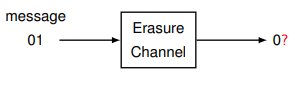
\includegraphics[scale=1.2]{22025-04-29.png}
    
\end{center}
f any bit is erased, there is no way to determine the original message (all hypothesis are equally possible).\\
So the goal here is the put redundancy, the goal is the create a redundancy that match exactly the message. The redundancy serves to deal with the back eyes (i don't rembeber).\\
So first we got rid of redundancy, we encrypt, and the finaly we add back in redundancy (which is not the same as the one we got rid off).
\\    
So first we got rid of redundancy, we encrypt, and the finaly we add back in redundancy (which is not the same as the one we got rid off).
\\
Now suppose that we do channel coding like this:
\begin{center}
    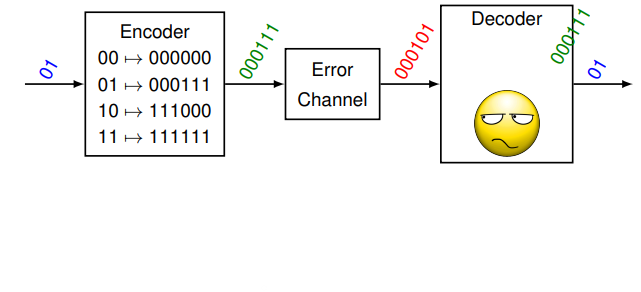
\includegraphics[scale=1]{32025-04-29.png}
\end{center}
The channel output is not a valid codeword. The decoders recognizes it, and assumes that the transmitted codeword is the one that agrees in most position with the observed channel output.\\
We add redundancy like some backups bits to make it stronger. 

\end{parag}
\begin{parag}{We study only block codes}
    The above is an $\left(n, k\right)$ \important{block code} with $n= 6$ and $k =  2$: each $k$ source symbols are substituted by $n$ channel symbols over the same alphabet.\\
    Since the alphabet is $\{0, 1\}$, we call it a \important{binary} $\left(n, k\right)$ block code.

    \begin{framedremark}
        We consider only bock codes
    \end{framedremark}
    
    
\end{parag}

\begin{parag}{Example}
    The following is a convolutional encoder: every encoder input symbol produces two encoder output symbols.\\
    The output pair produced at any given time is a linear function of the corresponding encoder input and encoder state (the previous two inputs).
    \begin{center}
        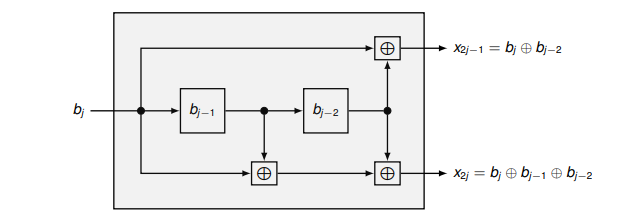
\includegraphics[scale=0.9]{42025-04-29.png}
    \end{center}
        So here we put the bit (from the encryption or whatever) we stores the previous bit. We then compute the two output.\\
        Here this is not a really good code (too slow for our smartphone but it is okay for satellite communications).

    
\end{parag}
\begin{parag}{Terminology}
    \begin{itemize}
        \item The code $\mathcal{C}$ is the set of codewords 
        \item A codeword $c$ is an element of $\mathcal{A}^n$. (the alphabet $\mathcal{A}$ is $\left\{0, 1\right\}$ in our example)
        \item The block length is $n$  (which is the length after the $\to$)
        \item Each codeword carries $k = \log_2\left|\mathcal{C}\right|$ bits of information (however we don't have to use $\log_2$ we can also use $\log_{\left|\mathcal{A}\right|}$ which won't have bit as a unit).
        \item The rate is $\frac{k}{n}$ bits per symbol
    \end{itemize}
    
   \begin{framedremark}
       Here $\left|\mathcal{C}\right|$ doesn't have to be equal to $\mathcal{A}^n$.
   \end{framedremark}
    
\end{parag}
\section{Hamming Distance}
\begin{parag}{Hamming distance}
    \begin{definition}
    The \important{Hamming distance $d\left(x, y\right)$} between two $n$-tuples $x$ and $y$ is the number of positions in which they differ.
    \end{definition}
    \begin{subparag}{Example}
        \begin{itemize}
            \item $x = \left(101110\right)$ ,  $y = \left(100110\right)$, $d\left(x, y\right) = 1$
            \item $x = \left(0427222\right)$, $y = \left(1227986\right)$, $d\left(x, y\right) = 5$
        \end{itemize}
        
    \end{subparag}
    
\end{parag}
\begin{parag}{The Hamming distance is indeed a distance}
    In math, a function of two variables is a distance if it satisfies the following axioms:
    \begin{definition}
        Distance axioms:
    \begin{itemize}
        \item \important{non-negativity}: $d\left(x, y\right) \geq 0$ with equality if and only if $x = y$
        \item \important{Symmetry}: $d\left(x, y\right) = d\left(y, x\right)$
        \item \important{triangle inequality}: $d\left(x, z\right) \leq d\left(x, y\right) + d\left(y, z\right)$
    \end{itemize}
    \end{definition}
    \begin{subparag}{Proof}
        We can first rewrite the distance like this:
        \begin{align*} d\left(x, y\right) = \sum_{i =  1}^{n} d\left(x_i, y_i\right) \end{align*}
        Where the $x_i$ and $y_i$ have a distance of $1$.\\
        The claim is: $d\left(x_i, z_i\right) \leq d\left(x_i, y_i\right) + d\left(y_i, z_i\right)$.\\
        To prove this we do a proof by cases:
       \begin{itemize}
           \item \important{Case 1}: $x_i = z_i \iff d\left(x_i, z_i\right) = 0$ there fore the inequality hold ( $ 0 \leq d\left(x_i, y_i\right) + d\left(y_i + z_i\right)$
           \item \important{Case 2}: $x_i \neq z_i \iff d\left(x_i, z_i\right) = 1$ \\Therefore in this case, there is at least one of the $d\left(x_i, y_i\right) = 1$ or $d\left(y_i, z_i\right)  1$ (or both) which is greater or equal to $1$. (here we use one because we said before that we were using ``vecteurs unitaires''.
       \end{itemize}
        

    \end{subparag}
\end{parag}

\begin{parag}{Minimum Distance decoder}
    
    \begin{itemize}
        \item The decoder guesses the encoder input based on the channel output
        \item Here we consider only \important{minimum distance decoders}.
    \end{itemize}
    \begin{center}
        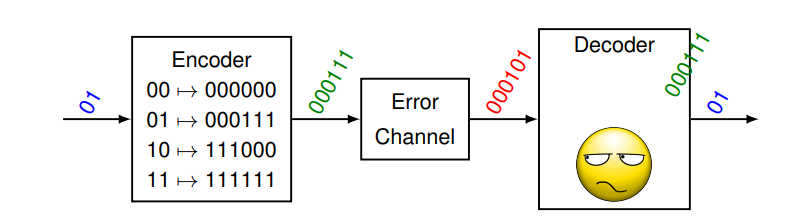
\includegraphics[scale=0.8]{52025-04-29.png}
    \end{center}
    
    How it works is pretty simple. It take the output codeword and compute the hamming distance with every element of the alphabet $\mathcal{C}$. And chose the one with the smallest hamming distance.\\
 For our example let us compute the hamming distance:
 \begin{align*} d_H\left(000101, 00000\right) = 2\\
 d_H\left(000101, 000111\right) = 1\\
d_H\left(000101, 111000\right) = 5\end{align*}
We called here $000111$ the winner! (we don't know for sure if it is \important{but} it is a good answer, a good starting point).
\end{parag}

\begin{parag}{Minimum distance decoder}
    \begin{definition}
        Let $y$ be the channel output observed by the decoder. A minimum-distance decoder decides that the channel input is (one of) the $\hat{c} \in \mathcal{C}$ for which $d\left(y, \hat{c}\right)$ is minimized.
        \begin{align*} \hat{c} \in \text{arg } \text{min}_{x \in \mathcal{C}}d\left(y, x\right)  \end{align*}
    \end{definition}
    We pick one in the minimum if there are more than one with small Hamming distance.\\
    The justification is that a small error weight is more likely than a large one.
\end{parag}
\begin{parag}{Minimum distance}
    \begin{definition}
    The minimum distance of a code $\mathcal{C}$ is
    \begin{align*} d_{min}\left(\mathcal{C}\right) = \text{min}_{x, y \in \mathcal{C}: x \neq y} d\left(x, y\right) \end{align*}
    \end{definition}
    \begin{subparag}{Example}
        Given the set $\mathcal{C} = \{000000, 100110, 011001, 111111\}$, we get that
        \begin{align*} d_{min}\left(\mathcal{C}\right) = 3 \end{align*}
    \end{subparag}
\end{parag}

\begin{parag}{What to expect from a decoder}
    For an error channel:
    \begin{itemize}
        \item Channel error correction: The best is if the decoder recognize and corrects the channel errors. In this case, the encoder input is recovered error-free.
        \item Channel-error detection: in some circumstances, the encoder is able to detect the presence channel errors but it is unable to correct them. The receiver may or may not ask for retransmission
        \item Decoding error: the worst is if the decoder tries to do as in (1) and makes the wrong decision.
    \end{itemize}
   For an erasure channel:
   \begin{itemize}
      \item erasure correction: the best is if the decoder is capable of filling in the erased positions. In this case, the encoder input is recovered error.free
      \item (erasure detection: unlike errors, erasure are always detected)
      \item decoding error: the worse is if the decoder fills in one or more erased position with incorrect symbols.
   \end{itemize}
   
\end{parag}
\begin{parag}{Error detection}
    The question now is how does error detection is related to $d_{min}\left(\mathcal{C}\right)$
    \begin{theoreme}
        \begin{enumerate}
            \item Channel errors of weight $p < d_{min}\left(\mathcal{C}\right)$ do not lead to a codeword. Hence they are detected.
            \item Some channel errors of weight $p \geq d_{min}\left(\mathcal{C}\right)$ do lead to another codeword. Hence they cannot be detected by a minimum-distance decoder.
        \end{enumerate}
        
    \end{theoreme}
    \begin{subparag}{Note}
        Erasures are always detected (by definition)
    \end{subparag}
    \begin{subparag}{Proof}
       Firstly, let $c \in \mathcal{C}$ be transmitted and $y$ be received. We know that if $p = d\left(c, y\right) < d_{min}\left(\mathcal{C}\right)$, $y$ cannot be a codeword, therefore the error is detected.\\ 
    We construct an example in which a channel error of weight $p = d_{min}\left(\mathcal{C}\right)$ cannot be detected.\\
    Let $c$ and $c'$ be a codeword at distance $d_{min}\left(\mathcal{C}\right)$.\\
    Suppose that $c$ is the channel input and the channel output is $y = c'$. \\
    $y$ is a codeword. A minimum distance decoder will decide that no channel error has occured.
    \end{subparag}
\end{parag}

\begin{parag}{Example (Error detection)}
    Let the encoding map be the MOD 97-10 procedure:
    \begin{align*} u \to v = \left(100 \cdot  u\right) + \left(98 - \left[100 \cdot  u\right]_{97}\right) \end{align*}
    Recall that $v$ is considered as valid if $\left[v\right]_{97} = 1$\\
    For example $u = 0216936631 \to v = 021693663165$
    Suppose $v$ is transmitted and $v'$ is received, $d\left(v, v'\right) = 1$.\\
    We can always write $v' = v + a10^k$ with $a \in \{-9, \ldots, -1, 1, \ldots, 9\}$.\\
    The only way for $v'$ to be a valid codeword is if $\left[a10^k\right]_{97} = 0$.\\
    Since $\left[10\right]_{97}$ is invertible, so is $\left[10^k\right]_{97}$, hence $a = 0$.\\
    Therefore all weight 1 errors are detected, implying that the minimum distance is at least $2$.
\end{parag}

